\documentclass[../../script.tex]{subfiles}
%! TEX root = ../../script.tex

\begin{document}
\section{Continuity}
\begin{center}
    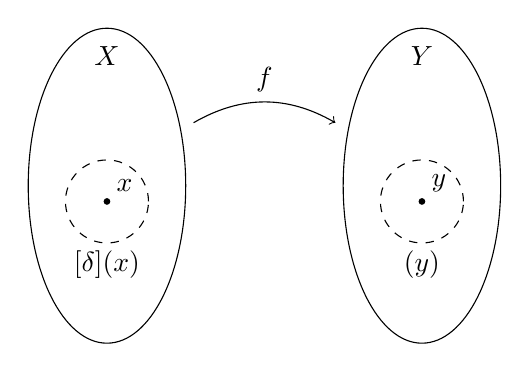
\begin{tikzpicture}
        \draw (-2, 0) ellipse (1cm and 2cm) node[above=1.4cm] (X) {$X$};
        \draw (2, 0) ellipse (1cm and 2cm) node[above=1.4cm] (Y) {$Y$};

        \draw [->] (-0.9, 0.8) to [out=30, in=150] node[above] {$f$} (0.9, 0.8);

        \draw[fill] (-2, -0.2) circle [radius=1pt] node[above right] {$x$};
        \draw[fill] (2, -0.2) circle [radius=1pt] node[above right] {$y$};

        \draw[dashed] (-2, -0.2) circle [radius=15pt] node[below=0.5cm] {$\oball[\delta](x)$};
        \draw[dashed] (2, -0.2) circle [radius=15pt] node[below=0.5cm] {$\oball(y)$};
    \end{tikzpicture}
\end{center}

\begin{defi}
    Let $(X, d_X), (Y, d_Y)$ be metric spaces. $f: x \rightarrow y$ is said to be continuous in $x \in X$ if 
    \[
        \forall \epsilon > 0 ~\exists \delta > 0: ~~\tilde{x} \in \oball[\delta](x) \implies f(\tilde{x}) \in \oball(f(x))
    \]
    $f$ is said to be continuous is it is continuous in every point.
\end{defi}

\begin{eg}
    \begin{enumerate}[(i)]
        \item Let $\metric$ be a metric space.
        \begin{align*}
            \idf: X &\longrightarrow X \\
            x &\longmapsto x
        \end{align*}
        is continuous (choose $\delta = \epsilon$).

        \item The function 
        \begin{align*}
            f: \realn^2 &\longrightarrow \realn^2 \\
            (x, y) &\longmapsto (x, -y)
        \end{align*}
        is continuous. For $(\tilde{x}, \tilde{y}), (x, y) \in \realn^2$ we have 
        \begin{align*}
            \norm{f(\tilde{x}, \tilde{y}) - f(x, y)}^2 &= \norm{(\tilde{x} - x, y - \tilde{y})}^2 = (\tilde{x} - x)^2 + (y - \tilde{y})^2 \\
            &= \norm{(\tilde{x}, \tilde{y}) - (x, y)}^2
        \end{align*}

        \item Consider 
        \begin{align*}
            f: \realn^2 &\longrightarrow \realn \\
            (x, y) &\longmapsto \begin{cases}
                0, &x \cdot y = 0 \\
                1, &x \cdot y \ne 0
            \end{cases}
        \end{align*}
        $f$ is non continuous in $(0, 0)$.
    \end{enumerate}
\end{eg}

\begin{rem}
    \begin{enumerate}[(i)]
        \item \[f \text{ continuous in } x \iff \forall \epsilon > 0 ~\exists \delta > 0: ~~f(\oball[\delta](x)) \subset \oball(f(x))\]
        \item Continuity is a local property, this means if $x \in X$, $U$ a neighbourhood of $x$ and $f, g$ functions with $f \vert_U = g \vert_U$, then 
        \[
            f \text{ continuous} \iff g \text{ continuous}
        \]
    \end{enumerate}
\end{rem}

\begin{thm}
    Let $x_0 \in X$, $g: X \rightarrow Y$ and $f: Y \rightarrow Z$. If $g$ is continuous in $x_0$ and $f$ is continuous in $g(x_0)$,
    then $f \circ g$ is continuous in $x_0$.

    \begin{center}
        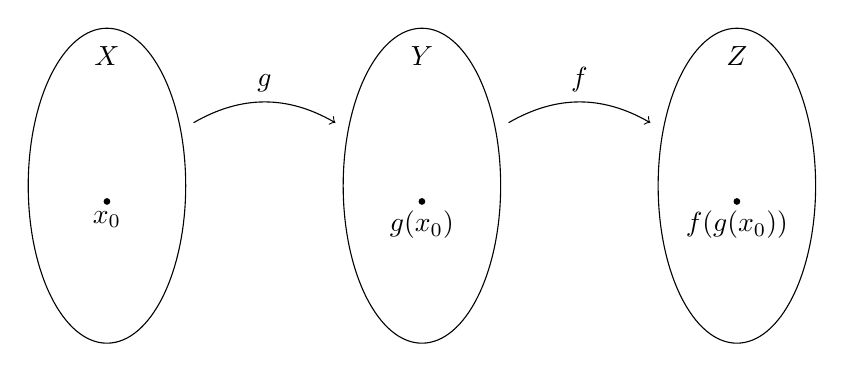
\begin{tikzpicture}
            \draw (-4, 0) ellipse (1cm and 2cm) node[above=1.4cm] {$X$};
            \draw (0, 0) ellipse (1cm and 2cm) node[above=1.4cm] {$Y$};
            \draw (4, 0) ellipse (1cm and 2cm) node[above=1.4cm] {$Z$};

            \draw [->] (-2.9, 0.8) to [out=30, in=150] node[above] {$g$} (-1.1, 0.8);
            \draw [->] (1.1, 0.8) to [out=30, in=150] node[above] {$f$} (2.9, 0.8);

            \draw[fill] (-4, -0.2) ellipse [radius=1pt] node[below] {$x_0$};
            \draw[fill] (0, -0.2) ellipse [radius=1pt] node[below] {$g(x_0)$};
            \draw[fill] (4, -0.2) ellipse [radius=1pt] node[below] {$f(g(x_0))$};
        \end{tikzpicture}
    \end{center}
\end{thm}
\begin{proof}
    Since $f, g$ are continuous we know that
    \begin{subequations}
        \begin{align}
            \forall \epsilon > 0 ~\exists \delta > 0&: ~~y \in \oball[\delta](g(x_0)) \implies f(y) \in \oball(f(g(x_0))) \\
            \forall \delta > 0 ~\exists \rho > 0&: ~~x \in \oball[\rho](x_0) \implies g(x) \in \oball[\delta](g(x_0))
        \end{align}
    \end{subequations}
    Then $\forall x \in \oball[\rho](x_0)$ we have 
    \begin{equation}
        (f \circ g)(x_0) = f(g(x_0)) \in \oball(f(g(x_0))) 
    \end{equation}
\end{proof}

\begin{defi}[Lipschitz continuity]
    A function $f: X \rightarrow Y$ is said to be Lipschitz continuous if
    \[
        \exists L > 0: ~~d_Y(f(x), f(y)) \le L \cdot D_X(x, y)
    \]
    $L$ is called Lipschitz constant. If $L = 1$, $f$ is called contraction.
\end{defi}

\begin{eg}
    Let $f, g: [0, 1] \rightarrow \realn$.
    \begin{align*}
        f(x) = x^2 && g(x) = \sqrt{x}
    \end{align*}
    $f$ is Lipschitz continuous, $g$ is not.
\end{eg}

\begin{thm}
    Every Lipschitz continuous function is continuous.
\end{thm}
\begin{proof}
    Let $f: X \rightarrow Y$ be Lipschitz continuous, with Lipschitz constant $L$. Let $\epsilon > 0$, 
    then for $x \in \oball[\frac{\epsilon}{L}](x_0)$
    \begin{equation}
        d(f(x), f(x_0)) \le L \cdot d(x, x_0) < \epsilon
    \end{equation}
    Thus, $f$ is continuous in $x_0$, and since we chose an arbitrary $x_0$, $f$ is continuous everywhere.
\end{proof}

\begin{eg}
    \begin{enumerate}[(i)]
        \item Consider 
        \begin{align*}
            \pi_i: \field^n &\longrightarrow \field \\
            (x_1, x_2, \cdots, x_n) &\longmapsto x_i
        \end{align*}
        Then 
        \[
            \abs{\pi_i(x) - \pi_i(y)} = \abs{x_i - y_i} \le \norm{x - y}
        \]
        So $\pi_i$ is a contraction.

        \item Let $(X, d), (X \times X, d_{X \times X})$ be metric spaces. Then 
        \begin{align*}
            d: X \times X &\longrightarrow \realn \\
            (x, y) &\longmapsto d(x, y)
        \end{align*}
        is a contraction. Let $x_1, x_2, y_1, y_2 \in X$ and apply the triangle inequality
        \[
            d(x_1, y_1) \le d(x_1, x_2) + d(x_2, y_1) \le d(x_1, x_2) + d(y_2, y_1) + d(x_2, y_2)
        \]
        This implies 
        \begin{align*}
            \abs{d(x_1, y_1) - d(x_2, y_2)} &\le d(x_1, x_2) + d(y_1, y_2) \\
            &= d_{X \times X} ((x_1, x_2), (y_1, y_2))
        \end{align*}
        which means the metric is continuous.

        \item Analogously, this works for $\dnorm$.
    \end{enumerate}
\end{eg}

\begin{thm}
    Let $f: X \rightarrow Y$.
    \[
        f \text{ is continuous in } x \in X \iff \substack{x \text{ is an isolated point in } X \\ \text{or } \limes{\tilde{x}}{x} f(\tilde{x}) = f(x)}
    \]
\end{thm}
\begin{proof}
    Let $f$ be continuous in $x \in X$. If $x$ is an isolated point there is nothing to show, so let $x$ be a limit point. Then 
    \begin{equation}
        \forall \epsilon > 0 ~\exists \delta > 0: ~~f(\tilde{x}) \in \oball(f(x)) ~~\forall \tilde{x} \in \oball[\delta](x)
    \end{equation}
    Now let $x$ be an isolated point, i.e. $\exists \delta > 0$ such that $\oball[\delta](x) = \set{x}$. Then 
    \begin{equation}
        f(\oball[delta](x)) = \set{f(x)} \subset \oball(f(x)) ~~\forall \epsilon > 0
    \end{equation}
    If $x$ is a limit point and $\limes{\tilde{x}}{x} f(\tilde{x}) = f(x)$, then let $\epsilon > 0$
    \begin{equation}
        \exists \delta > 0: ~~f(\dot{\oball[\delta]}(x)) \subset \oball(f(x))
    \end{equation}
    This then implies 
    \begin{equation}
        f(\oball[\delta]) \subset \oball(f(x))
    \end{equation}
\end{proof}

\begin{cor}
    \[
        f: X \rightarrow Y \text{ continuous in } x \in X \iff \forall \anyseqdef{X}: ~~f(x_n) \conv{x_n \rightarrow x} f(x)
    \] 
    This means, for continuous $f$ we have 
    \[
        \limn f(x_n) = f(\limn x_n)
    \]
\end{cor}

\begin{cor}
    Let $f_1, \cdots, f_n: \realn^m \rightarrow \real$. Then define
    \begin{align*}
        f: \realn^m &\longrightarrow \realn^n \\
        x &\longmapsto \left( f_1(x), f_2(x), \cdots, f_n(x) \right)
    \end{align*}
    $f$ is continuous if and only if $f_1, \cdots, f_n$ are continuous.
\end{cor}

\begin{cor}
    Let $f, g: X \rightarrow \realn$ be continuous in $x \in X$. Then 
    \begin{align*}
        f + g && f \cdot g 
    \end{align*}
    are continuous in $x$, and if $g(x) \ne 0$ then 
    \[
        \frac{f}{g}
    \]
    is also continuous in $x$.
\end{cor}

\begin{eg}
    Let $\eta = (\eta_1, \cdots, \eta_n) \in \natn_0^n$ and $x \in \field^n$. Define 
    \[
        x^{\eta} = x_1^{\eta_1} \cdot x_2^{\eta_2} \cdot x_3^{\eta_3} \cdot \cdots \cdot x_n^{\eta_n}
    \]
    $\eta$ is called multi index. We set
    \[
        \abs{\eta} := \eta_1 + \eta_2 + \eta_3 + \cdots + \eta_n
    \]
    Let $c_{\eta} \in \field ~~\forall \eta$ with $\abs{\eta} \le N ~~N \in \natn$. Then we call 
    \begin{align*}
        f: \field^n &\longrightarrow \field \\
        x &\longmapsto \sum_{|\eta| \le N} c_{\eta} \cdot x^{\eta}
    \end{align*}
    a polynomial with $n$ variables. Such polynomials are continuous. Example:
    \[
        (x_1, x_2) \longmapsto x_1^2 + x_2^2 + x_1^9 + x_2^{17}
    \]
\end{eg}

\begin{rem}
    In the context of polynomials (and power series) we define 
    \[
        0^0 = 1
    \]
    Reminder: If $f: X \rightarrow Y$ and $U \subset Y$ then $\inv{f}(U)$ is said to be the preimage of $U$ under $f$.
    It's the set of all points of $X$ that get mapped to $U$.
    \[
        \inv{f}(U) = \set[f(x) \in U]{x \in X}
    \]
\end{rem}

\begin{thm}
    Let $f: X \rightarrow Y$
    \begin{enumerate}[(i)]
        \item 
        \[
            f \text{ is continuous in } x \iff \substack{\inv{f}(U) \text{ is a neighbourhood of} \\ x ~~\forall U \text{neighbourhood of } f(x)}
        \]

        \item 
        \[
            f \text{ is continuous} \iff \inv{f}(O) \text{ is open } \forall O \subset Y \text{ open}
        \]

        \item 
        \[
            f \text{ is continuous} \iff \inv{f}(C) \text{ is closed } \forall C \subset Y \text{ closed}
        \]
    \end{enumerate}
\end{thm}
\begin{proof}
    We will prove (i). Let $U$ be a neighbourhood of $f(x)$, i.e.
    \begin{equation}
        \exists \epsilon > 0: ~~\oball(f(x)) \subset U
    \end{equation}
    Since $f$ is continuous
    \begin{equation}
        \exists \delta > 0: ~~f(\oball[\delta](x)) \subset \oball(f(x))
    \end{equation}
    which in turn means 
    \begin{equation}
        \oball[\delta](x) \subset \inv{f}(\oball(f(x))) \subset \inv{f}(U)
    \end{equation}
    so $\inv{f}(U)$ is a neighbourhood of $f(x)$. Now let $\epsilon > 0$. 
    Since $\oball(f(x))$ is a neighbourhood of $f(x)$, $\inv{f}(\oball(f(x)))$ is a neighbourhood of $x$. This means 
    \begin{equation}
        \exists \delta > 0: ~~\oball[\delta](x) \subset \inv{f}(\oball(f(x)))
    \end{equation}
    Thus $f(\oball[\delta](x)) \subset \oball(f(x))$ which means $f$ is continuous in $x$.

    (ii) and (iii) are left to the reader.
\end{proof}

\begin{defi}[Subsequences and (sequential) compactness]
    Let $\metric$ be a metric space, and $\anyseqdef{X}$, $(n_k) \subset \natn$ are strictly monotonically increasing. 
    Then $(x_{n_k})$ is said to be a subsequence of $(x_n)$.

    A subset $A \subset X$ is said to be (sequentially) compact, if every sequence $\seq{x} \subset A$ has a subsequence convergent in $A$.
\end{defi}

\begin{rem}
    If $\seq{x}$ converges to $x \in X$, then every subsequence of $\seq{x}$ converges to $x$. However, consider 
    \[
        \seq{x} = (-1)^n
    \]
    This sequence doesn't converge, but the subsequences $(x_{2n})$ and $(x_{2n + 1})$ converge to (different) values.
\end{rem}

\begin{eg}
    Let $X = \realn$, then $(0, 1)$ and $\natn$ are not compact. Because
    \begin{align*}
        (x_n = \frac{1}{n}) \subset (0, 1) && (x_n = n) \subset \natn
    \end{align*}
    have no convering subsequences.
\end{eg}

\begin{thm}
    \[
        A \subset \realn^n \text{ is compact} \iff A \text{ closed and bounded}
    \]
\end{thm}
\begin{proof}
    Assume $A$ is not  closed, i.e. for $x \in \boundary{A} \setminus A$
    \begin{equation}
        \exists \anyseqdef{A} \text{ with } x_n \conv{} x
    \end{equation}
    Every subequence of $\seq{x}$ converges to $x$, but $x \ne  A$. From this follows that $A$ is not compact.
    Assume $A$ is not bounded, i.e. $A \setminus \oball[n](0) \ne \varnothing ~~\forall n \in \natn$. Now choose 
    $\anyseqdef{A}$ such that $\norm{\seq{x}} \ge n$. $\seq{x}$ cannot have a convergent subsequence, because on the one hand 
    for $(x_{n_k})$ convergent to $x$ we have $\norm{x_{n_k}} \rightarrow \norm{x}$, but on the other hand 
    $\norm{x_{n_k}} \ge n_k \longrightarrow \infty$. This proves the "$\implies$" direction, to prove the inverse, consider the case $n = 1$:
    Let $A \subset \realn$ be bounded and closed. Then 
    \begin{equation}
        \exists K > 0: ~~A \subset I_1 = [-K, K]
    \end{equation}
    Let $\anyseqdef{A}$ be a sequence. We recursively define more intervals. Let $I_k = [a, b)$ such that $x_n \in I_k$ for infinitely many $n \in \natn$.
    Half the interval:
    \begin{subequations}
        \begin{align}
            I_{k+1} = \left[a, \frac{b - a}{2}\right) && \text{or} && I_{k+1} = \left[\frac{b - a}{2}, b\right)
        \end{align}
    \end{subequations}
    such that $x_n \in I_{k+1}$ for infinitely many $n \in \natn$. By doing this we are creating a sequence of nested intervals of length $K \cdot 2^{-k + 2}$.
    Now set $n_1 = 1$, and then recursively define
    \begin{equation}
        n_{k+1} > \max\set{n_1, \cdots, n_k} \text{ and } x_{n_{k+1}} \in I_{k + 1}
    \end{equation}
    We now need to show that $(x_{n_k})$ is convergent. Apply the Cauchy criterion: For $l > k$ we know that $x_{n_k}$ and $x_{n_l} \in I_k$, i.e.
    \begin{equation}
        \abs{x_{n_k} - x_{n_l}} \le K \cdot 2^{-k + 2} \conv{k \rightarrow \infty} 0
    \end{equation}
    This means, $x_{n_k}$ is a Cauchy sequence, so it converges to $x \in \realn$. Since $A$ is closed, we have $x \in A$.
\end{proof}

\begin{thm}
    Continuous mappings map compact sets to compact sets.
\end{thm}
\begin{proof}
    Let $f: X \rightarrow Y$ be continuous and $A \subset X$ compact. Let $\seq{x} \subset f(A)$. We need to show that $\seq{x}$ has a convergent subsequence.
    We know that 
    \begin{equation}
        \exists \anyseqdef[y]{A}: ~~x_n = f(y_n)
    \end{equation}
    Since $A$ is compact, there must be subsequences $(y_{n_k})$ with $y_{n_k} \conv{k \rightarrow \infty} y \in A$. Because of the continuity of $f$, we have 
    \begin{equation}
        \underbrace{f(y_{n_k})}_{x_{n_k}} \conv{} f(y) \in f(A)
    \end{equation}
    Thus, $f(A)$ is compact.
\end{proof}

\begin{rem}
    Let $f: \realn^n \rightarrow \realn^n$ be a continuous mapping. $f$ maps closed, bounded sets to closed, bounded sets.
    In general, closed sets are NOT mapped to closed sets, and bounded sets are NOT mapped to bounded sets.

    Example: $f: (0, \infty) \rightarrow \realn, ~~x \mapsto \inv{x}$
    \begin{align*}
        f(\underbrace{(0, 1)}_{\text{bounded}}) = \underbrace{(1, \infty)}_{\text{unbounded}} 
        && f(\underbrace{[1, \infty]}_{\text{closed}}) = \underbrace{(0, 1]}_{\text{not closed}}
    \end{align*}
\end{rem}

\begin{cor}
    Let $A \subset \realn^n$ be compact and $f: A \rightarrow \realn$ continuous. Then $f$ assumes its maximum on $A$. I.e.
    \[
        \exists x \in A: ~~f(y) \le f(x) ~~\forall y \in A
    \]
\end{cor}
\begin{proof}
    $f(A)$ is compact, so it's closed and bounded. We want to show that compact subsets $K$ of $\realn$ have a maximum $M := \sup K$
    such that $x_n \conv{} M$. Since $K$ is closed we know that $M \in \field$, so $M$ is a maximum.
    Especially, $\exists z \in f(A)$ maximum and $\exists x \in A$ with $f(x) = z$
\end{proof}

\begin{thm}
    Let $A \subset \realn^n, B \subset \realn^m$ be compact subsets and $f: A \rightarrow B$ a bijective, continuous mapping. 
    Then $\inv{f}$ is also continuous.
\end{thm}
\begin{proof}
    Define $g := \inv{f}$.  $g$ is also bijective and maps $B \rightarrow A$. Let $C \subset A$ be closed. 
    Since $A$ is bounded, $C$ is also bounded. Thus, $f(C)$ is also compact (i.e. bounded and closed), and we have 
    \begin{equation}
        \begin{split}
            f(C) &= \set[x \in C]{f(x) \in B} \\
            &= \set[g(y) \in C]{f(g(y)) \in B} \\
            &= \set[g(y) \in C]{y \in B} = \inv{g}(C)
        \end{split}
    \end{equation}
    So $\inv{g}(C)$ is bounded, and since $C$ was an arbitrary closed set, $g$ is also continuous.
\end{proof}
\end{document}